% Options for packages loaded elsewhere
% Options for packages loaded elsewhere
\PassOptionsToPackage{unicode}{hyperref}
\PassOptionsToPackage{hyphens}{url}
\PassOptionsToPackage{dvipsnames,svgnames,x11names}{xcolor}
%
\documentclass[
  10pt,
  letterpaper,
  DIV=11,
  numbers=noendperiod]{scrartcl}
\usepackage{xcolor}
\usepackage{amsmath,amssymb}
\setcounter{secnumdepth}{5}
\usepackage{iftex}
\ifPDFTeX
  \usepackage[T1]{fontenc}
  \usepackage[utf8]{inputenc}
  \usepackage{textcomp} % provide euro and other symbols
\else % if luatex or xetex
  \usepackage{unicode-math} % this also loads fontspec
  \defaultfontfeatures{Scale=MatchLowercase}
  \defaultfontfeatures[\rmfamily]{Ligatures=TeX,Scale=1}
\fi
\usepackage{lmodern}
\ifPDFTeX\else
  % xetex/luatex font selection
\fi
% Use upquote if available, for straight quotes in verbatim environments
\IfFileExists{upquote.sty}{\usepackage{upquote}}{}
\IfFileExists{microtype.sty}{% use microtype if available
  \usepackage[]{microtype}
  \UseMicrotypeSet[protrusion]{basicmath} % disable protrusion for tt fonts
}{}
% Make \paragraph and \subparagraph free-standing
\makeatletter
\ifx\paragraph\undefined\else
  \let\oldparagraph\paragraph
  \renewcommand{\paragraph}{
    \@ifstar
      \xxxParagraphStar
      \xxxParagraphNoStar
  }
  \newcommand{\xxxParagraphStar}[1]{\oldparagraph*{#1}\mbox{}}
  \newcommand{\xxxParagraphNoStar}[1]{\oldparagraph{#1}\mbox{}}
\fi
\ifx\subparagraph\undefined\else
  \let\oldsubparagraph\subparagraph
  \renewcommand{\subparagraph}{
    \@ifstar
      \xxxSubParagraphStar
      \xxxSubParagraphNoStar
  }
  \newcommand{\xxxSubParagraphStar}[1]{\oldsubparagraph*{#1}\mbox{}}
  \newcommand{\xxxSubParagraphNoStar}[1]{\oldsubparagraph{#1}\mbox{}}
\fi
\makeatother


\usepackage{longtable,booktabs,array}
\usepackage{calc} % for calculating minipage widths
% Correct order of tables after \paragraph or \subparagraph
\usepackage{etoolbox}
\makeatletter
\patchcmd\longtable{\par}{\if@noskipsec\mbox{}\fi\par}{}{}
\makeatother
% Allow footnotes in longtable head/foot
\IfFileExists{footnotehyper.sty}{\usepackage{footnotehyper}}{\usepackage{footnote}}
\makesavenoteenv{longtable}
\usepackage{graphicx}
\makeatletter
\newsavebox\pandoc@box
\newcommand*\pandocbounded[1]{% scales image to fit in text height/width
  \sbox\pandoc@box{#1}%
  \Gscale@div\@tempa{\textheight}{\dimexpr\ht\pandoc@box+\dp\pandoc@box\relax}%
  \Gscale@div\@tempb{\linewidth}{\wd\pandoc@box}%
  \ifdim\@tempb\p@<\@tempa\p@\let\@tempa\@tempb\fi% select the smaller of both
  \ifdim\@tempa\p@<\p@\scalebox{\@tempa}{\usebox\pandoc@box}%
  \else\usebox{\pandoc@box}%
  \fi%
}
% Set default figure placement to htbp
\def\fps@figure{htbp}
\makeatother


% definitions for citeproc citations
\NewDocumentCommand\citeproctext{}{}
\NewDocumentCommand\citeproc{mm}{%
  \begingroup\def\citeproctext{#2}\cite{#1}\endgroup}
\makeatletter
 % allow citations to break across lines
 \let\@cite@ofmt\@firstofone
 % avoid brackets around text for \cite:
 \def\@biblabel#1{}
 \def\@cite#1#2{{#1\if@tempswa , #2\fi}}
\makeatother
\newlength{\cslhangindent}
\setlength{\cslhangindent}{1.5em}
\newlength{\csllabelwidth}
\setlength{\csllabelwidth}{3em}
\newenvironment{CSLReferences}[2] % #1 hanging-indent, #2 entry-spacing
 {\begin{list}{}{%
  \setlength{\itemindent}{0pt}
  \setlength{\leftmargin}{0pt}
  \setlength{\parsep}{0pt}
  % turn on hanging indent if param 1 is 1
  \ifodd #1
   \setlength{\leftmargin}{\cslhangindent}
   \setlength{\itemindent}{-1\cslhangindent}
  \fi
  % set entry spacing
  \setlength{\itemsep}{#2\baselineskip}}}
 {\end{list}}
\usepackage{calc}
\newcommand{\CSLBlock}[1]{\hfill\break\parbox[t]{\linewidth}{\strut\ignorespaces#1\strut}}
\newcommand{\CSLLeftMargin}[1]{\parbox[t]{\csllabelwidth}{\strut#1\strut}}
\newcommand{\CSLRightInline}[1]{\parbox[t]{\linewidth - \csllabelwidth}{\strut#1\strut}}
\newcommand{\CSLIndent}[1]{\hspace{\cslhangindent}#1}



\setlength{\emergencystretch}{3em} % prevent overfull lines

\providecommand{\tightlist}{%
  \setlength{\itemsep}{0pt}\setlength{\parskip}{0pt}}



 


\usepackage{booktabs}
\usepackage{caption}
\usepackage{longtable}
\usepackage{colortbl}
\usepackage{array}
\usepackage{anyfontsize}
\usepackage{multirow}
\usepackage{xcolor, soul}
\definecolor{Light}{gray}{.90}
\sethlcolor{Light}
\let\OldTexttt\texttt
\renewcommand{\texttt}[1]{\OldTexttt{\hl{#1}}}
\usepackage{caption}
\captionsetup{font=small, labelfont=bf}
\setlength{\parindent}{0pt}
\setlength{\parskip}{1.25ex}
% Symbols %%%%%%%%%%%%%%%%%%%%%%%%%%%%%%%%%%%%%%%%%%%%%%%%%%%%%

\usepackage{amsthm}
\usepackage{amsmath}
\usepackage{amssymb}
\usepackage{amsfonts}

% New commands %%%%%%%%%%%%%%%%%%%%%%%%%%%%%%%%%%%%%%%%%%%%%%%%

% General mathematical symbols
% argmin help from egreg from tex.stackexchange.com/questions/5223
\newcommand{\R}{\mathbb{R}}
\newcommand{\onedim}{\mathbb{R}}
\newcommand{\ddim}{\mathbb{R}^d}
\newcommand{\kdim}{\mathbb{R}^k}

\newcommand{\eps}{\varepsilon}
\newcommand{\seq}[1]{\{ #1_{n} \}}

\DeclareMathOperator*{\sign}{sign}
\DeclareMathOperator*{\argmin}{arg\,min}
\DeclareMathOperator*{\argmax}{arg\,max}

% boldface
\newcommand{\bfH}{\mathbf{H}}
\newcommand{\bfI}{\mathbf{I}}
\newcommand{\bfO}{\mathbf{O}}
\newcommand{\bfU}{\mathbf{U}}
\newcommand{\bfu}{\mathbf{u}}
\newcommand{\bfV}{\mathbf{V}}
\newcommand{\bfv}{\mathbf{v}}
\newcommand{\bfW}{\mathbf{W}}
\newcommand{\bfw}{\mathbf{w}}
\newcommand{\bfG}{\mathbf{G}}
\newcommand{\bfX}{\mathbf{X}}
\newcommand{\bfx}{\mathbf{x}}
\newcommand{\bfY}{\mathbf{Y}}
\newcommand{\bfy}{\mathbf{y}}
\newcommand{\bfZ}{\mathbf{Z}}
\newcommand{\bfz}{\mathbf{z}}
\newcommand{\bfmu}{\boldsymbol{\mu}}
\newcommand{\bfeps}{\boldsymbol{\epsilon}}
\newcommand{\bfbeta}{\boldsymbol{\beta}}
\newcommand{\bfgamma}{\boldsymbol{\gamma}}
\newcommand{\bfS}{\mathbf{S}}
\newcommand{\bfB}{\mathbf{B}}

% Sets
\newcommand{\setA}{\mathcal{A}}
\newcommand{\setB}{\mathcal{B}}
\newcommand{\setC}{\mathcal{C}}
\newcommand{\setF}{\mathcal{F}}
\newcommand{\rademacher}{\mathcal{R}}
\newcommand{\setP}{\mathcal{P}}

% General stats
\newcommand{\E}{\mathbb{E}}
\DeclareMathOperator*{\var}{Var}
\DeclareMathOperator*{\cor}{Corr}
\DeclareMathOperator*{\cov}{Cov}
\newcommand{\prob}{\mathbb{P}}

\newcommand{\indep}{\perp \!\!\! \perp}
\newcommand{\depen}{\cancel{\indep}}
\newcommand{\indic}{\mathbbm{1}}
\newcommand{\Xbar}{\overline{X}_n}
\newcommand{\Xsqbar}{\overline{X^2_n}}
\newcommand{\Xbarsq}{\overline{X}^2_n}
\newcommand{\Ybar}{\overline{Y}_n}
\newcommand{\lik}{\mathcal{L}}
\newcommand{\ton}[1]{#1_1, \dots, #1_n}
\newcommand{\fisher}{\mathcal{I}}
\newcommand{\sumn}{\sum_{i = 1}^n}
\newcommand{\prodn}{\prod_{i = 1}^n}

% Distributions
\newcommand{\hpp}{\textrm{HPP}}
\newcommand{\ipp}{\textrm{IPP}}
\newcommand{\geom}{\textrm{Geom}}
\newcommand{\iid}{\overset{\textrm{i.i.d.}}{\sim}}
\newcommand{\pois}{\textrm{Pois}}
\newcommand{\bern}{\textrm{Bern}}
\newcommand{\N}{\mathcal{N}}
\newcommand{\MVN}{\textrm{MVN}}
\newcommand{\unif}{\textrm{Unif}}
\newcommand{\binomial}{\textrm{Binom}}
\newcommand{\expo}{\textrm{Expo}}
\newcommand{\hgeom}{\textrm{HGeom}}

\KOMAoption{captions}{tableheading}
\makeatletter
\@ifpackageloaded{caption}{}{\usepackage{caption}}
\AtBeginDocument{%
\ifdefined\contentsname
  \renewcommand*\contentsname{Table of contents}
\else
  \newcommand\contentsname{Table of contents}
\fi
\ifdefined\listfigurename
  \renewcommand*\listfigurename{List of Figures}
\else
  \newcommand\listfigurename{List of Figures}
\fi
\ifdefined\listtablename
  \renewcommand*\listtablename{List of Tables}
\else
  \newcommand\listtablename{List of Tables}
\fi
\ifdefined\figurename
  \renewcommand*\figurename{Figure}
\else
  \newcommand\figurename{Figure}
\fi
\ifdefined\tablename
  \renewcommand*\tablename{Table}
\else
  \newcommand\tablename{Table}
\fi
}
\@ifpackageloaded{float}{}{\usepackage{float}}
\floatstyle{ruled}
\@ifundefined{c@chapter}{\newfloat{codelisting}{h}{lop}}{\newfloat{codelisting}{h}{lop}[chapter]}
\floatname{codelisting}{Listing}
\newcommand*\listoflistings{\listof{codelisting}{List of Listings}}
\makeatother
\makeatletter
\makeatother
\makeatletter
\@ifpackageloaded{caption}{}{\usepackage{caption}}
\@ifpackageloaded{subcaption}{}{\usepackage{subcaption}}
\makeatother
\usepackage{bookmark}
\IfFileExists{xurl.sty}{\usepackage{xurl}}{} % add URL line breaks if available
\urlstyle{same}
\hypersetup{
  pdftitle={Comparison of randomized dichotomies and pairwise sample distances in between-sample comparisons},
  pdfauthor={Al Xin},
  colorlinks=true,
  linkcolor={blue},
  filecolor={Maroon},
  citecolor={Blue},
  urlcolor={Blue},
  pdfcreator={LaTeX via pandoc}}


\title{Comparison of randomized dichotomies and pairwise sample
distances in between-sample comparisons}
\author{Al Xin}
\date{Sep 10, 2026}
\begin{document}
\maketitle


\section{Shrinkage covariance
estimator}\label{shrinkage-covariance-estimator}

The standard multivariate covariance estimator cannot be applied in the
Mahalanobis distance calculation because the number of repetitions (6
for each image) is lower than the number of sites typically used to
evaluate separation.

However, one can apply a shrinkage approach, described in Schafer and
Strimmer {[}1{]} and based on a lemma proposed by Ledoit and Wolf
{[}2{]}. This approach is implemented in the R package \texttt{corpcor}.
Furthermore, \texttt{corpcor} handily provides \texttt{invcov.shrink()},
which directly calculates \(\boldsymbol{\Sigma}^{-1}\) rather than
estimating then inverting \(\boldsymbol{\Sigma}\) {[}3{]}.

Briefly, let \(\boldsymbol{\psi} = (\psi_1, \dots, \psi_p)\) be the
parameters of an unrestricted high-dimensional model of interest and let
\(\boldsymbol{\theta}\) be the parameters of a lower dimensional
restricted sub-model. e.g., \(\boldsymbol{\psi}\) is the mean vector of
a multivariate Normal and \(\boldsymbol{\theta}\) is the vector of a
contrained submodel where the means are all assumed to be equal. Then,
the linear shrinkage approach finds the new estimator \[
\boldsymbol{\psi}^* = \lambda \hat{\boldsymbol{\theta}} + (1 - \lambda) \hat{\boldsymbol{\psi}} : \lambda \in [0, 1]
\] where the optimal value \(\lambda^*\) can be found analytically by
optimizing \[
\lambda^* = 
\frac
{\sum_{i = 1}^p \left( \var (\hat\psi_i) - \cov (\hat\theta_i, \hat\psi_i) \right)}
{\sum_{i = 1}^p \E [(\hat\theta_i - \hat\psi_i)^2]}
\]

In the \texttt{corpcor} implementation, the shrinkage target (i.e., the
parameters of the constrained model) is taken as a diagonal covariance
matrix whose diagonal entries may be unequal, which shrinks the
off-diagonal elements of the estimated covariance matrix {[}1{]}. This
also produces a positive definite covariance estimate, as a convex
combination of a positive definite matrix and positive semidefinite
matrix yields a positive definite matrix.

\section{Pairwise samples compared with randomized
dichotomies}\label{pairwise-samples-compared-with-randomized-dichotomies}

Pairwise sample comparisons are done separately for each family. For
consistency, I'll use the same sites in the last notebook
(\texttt{20260826}).

Visually, the distributions between the pairwise sample comparisons and
the randomized dichotomies look similar, though the magnitudes of the
distances are affected by the different number of samples
(Figure~\ref{fig-rd_vs_ps}). The orderings on family-separated results
are also similar (these plots are saved but not rendered here). When
plotting the within-family averages and standard deviations against each
other (Figure~\ref{fig-rd_vs_ps_corr}), the correlations tend to be good
for within-family averages and worse for within-family standard
deviations (Table~\ref{tbl-rd_vs_ps}).

To make this more rigorous, one could test for similarity between the
relative rankings of region performance with a post hoc test. However,
this is probably overkill for now.

I am fairly unworried about big differences between the results from the
pairwise sample distances and the randomized dichotomies. Subsequent
analyses will be performed on the pairwise sample distances, which will
save time (and memory).

\begin{figure}

\centering{

\pandocbounded{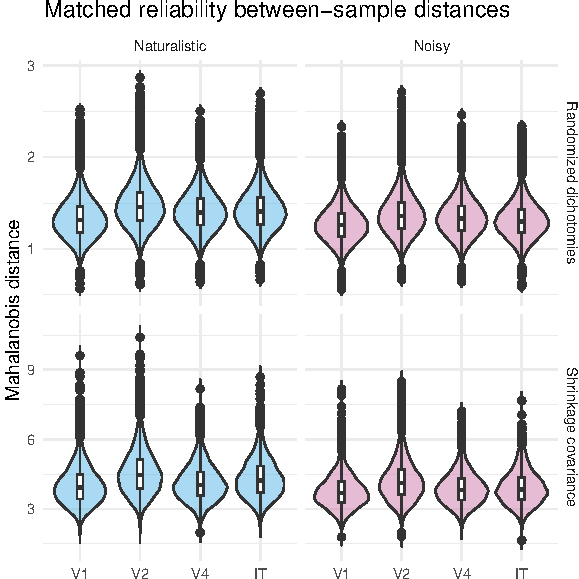
\includegraphics[keepaspectratio]{20260909_files/figure-pdf/fig-rd_vs_ps-1.pdf}}

}

\caption{\label{fig-rd_vs_ps}Violin plots comparing the distributions of
Mahalanobis distances for the randomized dichotomies approach (top) and
the pairwise between-sample distances found with the Ledoit-Wolf
shrinkage estimator.}

\end{figure}%

\begin{figure}

\centering{

\pandocbounded{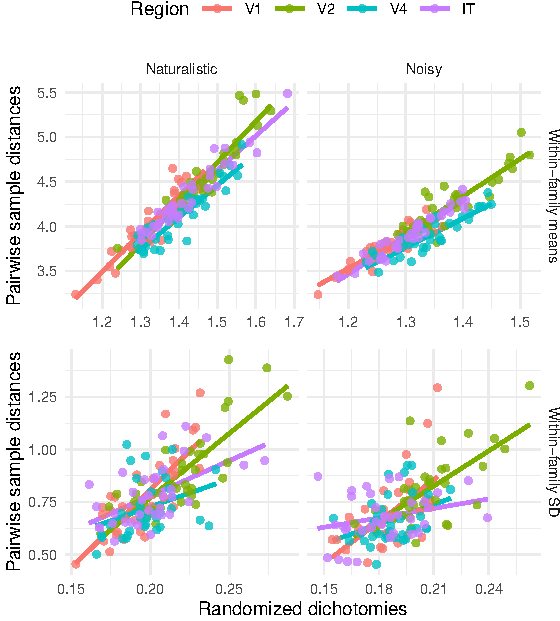
\includegraphics[keepaspectratio]{20260909_files/figure-pdf/fig-rd_vs_ps_corr-1.pdf}}

}

\caption{\label{fig-rd_vs_ps_corr}Comparison of summary statistics of
the distances found with pairwise sample distances and randomized
dichotomies. Means and standard deviations are calculated within each
texture family. The within-family means tend to show more correlation
across all regions. The correlation between the pairwise sample and
randomized dichotomies standard deviations is worse in IT than other
regions.}

\end{figure}%

\begin{table}

\caption{\label{tbl-rd_vs_ps}The correlations between family-wise
summary statistics of mean and standard deviation for each region and in
naturalistic or noisy families. The correlations of family-wise means
tends to be high for both types of texture families. Correlations in
within-family SD tend to drop in noisy families.}

\centering{

\fontsize{8.0pt}{10.0pt}\selectfont
\begin{tabular*}{\linewidth}{@{\extracolsep{\fill}}crrrr}
\toprule
 & \multicolumn{2}{c}{{Naturalistic}} & \multicolumn{2}{c}{{Noisy}} \\ 
\cmidrule(lr){2-3} \cmidrule(lr){4-5}
Region & Corr(Means) & Corr(SD) & Corr(Means) & Corr(SD) \\ 
\midrule\addlinespace[2.5pt]
V1 & 0.929 & 0.785 & 0.892 & 0.590 \\ 
V2 & 0.922 & 0.794 & 0.898 & 0.682 \\ 
V4 & 0.919 & 0.344 & 0.908 & 0.357 \\ 
IT & 0.957 & 0.578 & 0.963 & 0.281 \\ 
\bottomrule
\end{tabular*}

}

\end{table}%

\section{References}\label{references}

\phantomsection\label{refs}
\begin{CSLReferences}{0}{1}
\bibitem[\citeproctext]{ref-schafer_shrinkage_2005}
\CSLLeftMargin{1. }%
\CSLRightInline{Juliane Schäfer, Korbinian Strimmer. A shrinkage
approach to large-scale covariance matrix estimation and implications
for functional genomics. Statistical Applications in Genetics and
Molecular Biology {[}Internet{]}. 2005 {[}cited 2026 Sep
9{]};4(1):1--32. Available from:
\url{https://ideas.repec.org//a/bpj/sagmbi/v4y2005i1n32.html}}

\bibitem[\citeproctext]{ref-ledoit_improved_2003}
\CSLLeftMargin{2. }%
\CSLRightInline{Olivier Ledoit, Michael Wolf. Improved estimation of the
covariance matrix of stock returns with an application to portfolio
selection. Journal of Empirical Finance. 2003 Dec 1;10(5):603--21.
doi:\href{https://doi.org/10.1016/S0927-5398(03)00007-0}{10.1016/S0927-5398(03)00007-0}}

\bibitem[\citeproctext]{ref-schafer_corpcor_2021}
\CSLLeftMargin{3. }%
\CSLRightInline{Juliane Schafer, Rainer Opgen-Rhein, Verena Zuber, Miika
Ahdesmaki, A. Pedro Duarte Silva, Korbinian Strimmer. Corpcor: Efficient
estimation of covariance and (partial) correlation {[}Internet{]}. 2021
{[}cited 2026 Sep 9{]}. Available from:
\url{https://cran.r-project.org/package=corpcor}}

\end{CSLReferences}




\end{document}
